\documentclass{article}
\usepackage{amsfonts, amsthm, amsmath, amssymb, mathtools, ulem, mathrsfs, physics, esint, siunitx, tikz-cd}
\usepackage{pdfpages, fullpage, color, microtype, cancel, textcomp, markdown, hyperref, graphicx}
\usepackage{enumitem}
\graphicspath{{./images/}}
\usepackage[english]{babel}
\usepackage[autostyle, english=american]{csquotes}
\MakeOuterQuote{"}
\usepackage{xparse}
\usepackage{tikz}
\usepackage{algpseudocode}

% fonts
\def\mbb#1{\mathbb{#1}}
\def\mfk#1{\mathfrak{#1}}
\def\mbf#1{\mathbf{#1}}
\def\tbf#1{\textbf{#1}}

% common bold letters
\def\bP{\mbb{P}}
\def\bC{\mbb{C}}
\def\bH{\mbb{H}}
\def\bI{\mbb{I}}
\def\bR{\mbb{R}}
\def\bQ{\mbb{Q}}
\def\bZ{\mbb{Z}}
\def\bN{\mbb{N}}

% brackets
\newcommand{\br}[1]{\left(#1\right)}
\newcommand{\sbr}[1]{\left[#1\right]}
\newcommand{\brc}[1]{\left\{#1\right\}}
\newcommand{\lbr}[1]{\left\langle#1\right\rangle}

% matrices
\newcommand{\m}[2][b]{\begin{#1matrix}#2\end{#1matrix}}
\newcommand{\arr}[3][\sbr]{#1{\begin{array}{#2}#3\end{array}}}
\DeclareMathOperator{\Span}{span}

% greek
\newcommand{\e}{\epsilon}
\newcommand{\p}{\varphi}
\renewcommand{\t}{\theta}

% misc
\NewDocumentCommand{\app}{O{x} O{\infty}}{\xrightarrow{#1\to#2}}
\newcommand{\sse}{\subseteq}
\renewcommand{\ss}{\subset}
\newcommand{\vn}{\varnothing}
\newcommand{\inv}{^{-1}}
\newcommand{\imp}{\implies}
\newcommand{\impleft}{\reflectbox{$\implies$}}
\renewcommand{\ip}[2]{\lbr{#1,#2}}
\renewcommand{\bar}{\overline}
\DeclareMathOperator{\cis}{cis}
\DeclareMathOperator{\Arg}{Arg}
\renewcommand{\d}{\partial}
\newcommand{\pf}{\tbf{Proof. }}
\renewcommand{\L}{\mathcal{L}}

% title
\title{Scientific Computing HW 7}
\author{Ryan Chen}
%\date{\today}
\setlength{\parindent}{0pt}


\begin{document}
	
\maketitle



\begin{enumerate}
	
	
	
	\item 
	
	\begin{enumerate}
		
		
		
		\item 
		
		
		
		\item
		
		
		
	\end{enumerate}
	
	
	
	\pagebreak
	
	
	
	\item Below, the level curve $\det A=0$ is colored red, and the level curve $\norm{A}_*=a$ is colored purple. We see that the curves indeed intersect at the corners of $\norm{A}_*=a$.
	
	\begin{center}
		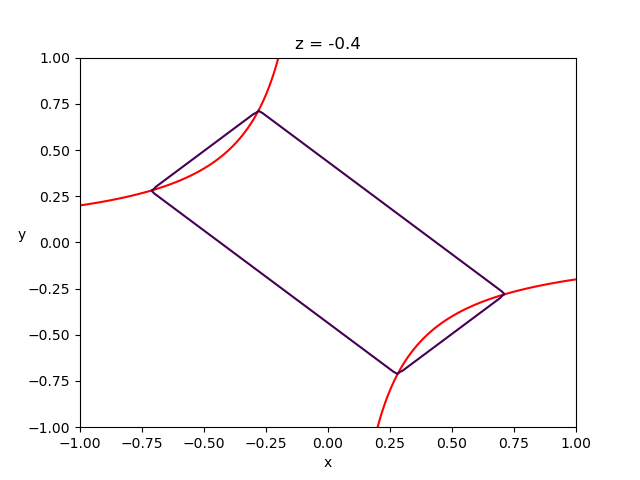
\includegraphics[scale=.3]{hw7 level curves z = -0.4}
		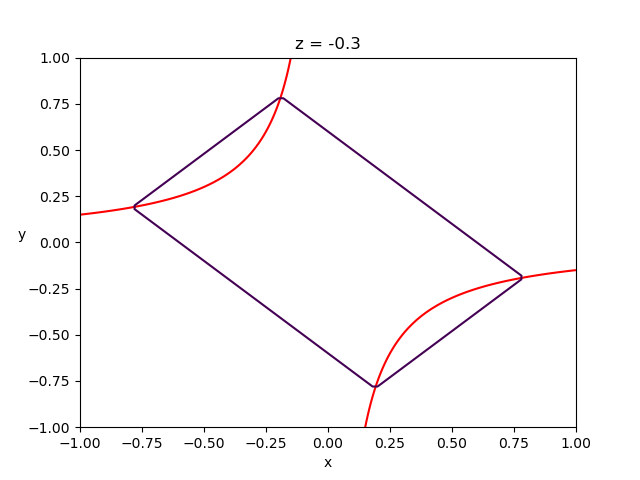
\includegraphics[scale=.3]{hw7 level curves z = -0.3}
		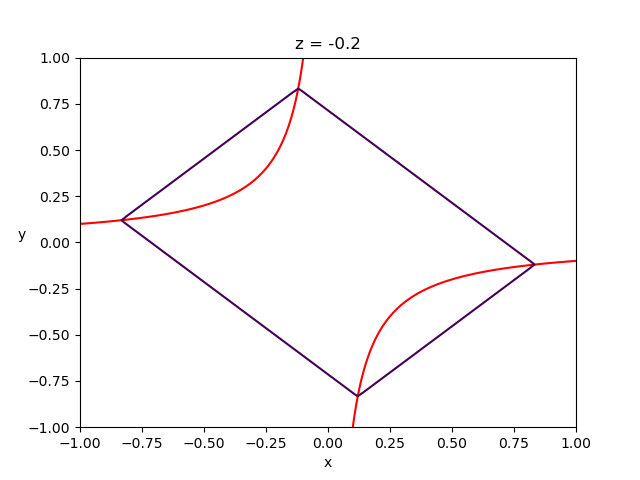
\includegraphics[scale=.3]{hw7 level curves z = -0.2}
		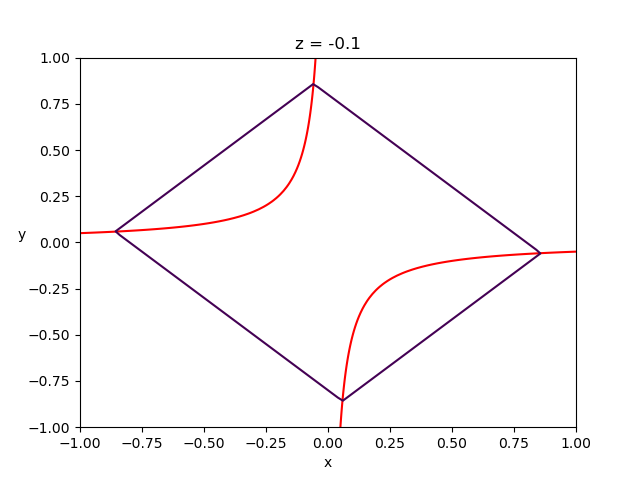
\includegraphics[scale=.3]{hw7 level curves z = -0.1}
		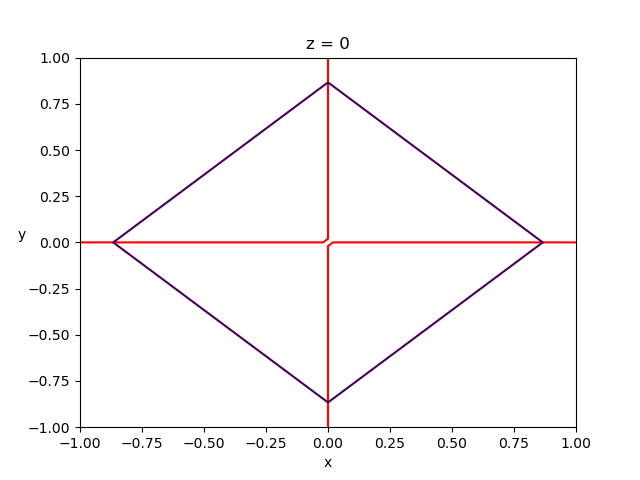
\includegraphics[scale=.3]{hw7 level curves z = 0}
		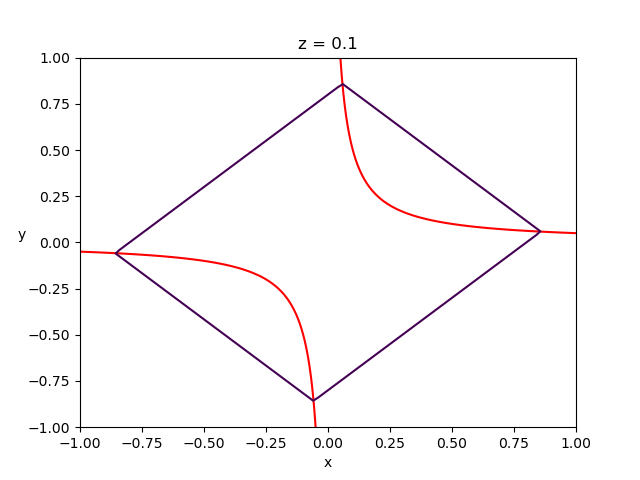
\includegraphics[scale=.3]{hw7 level curves z = 0.1}
		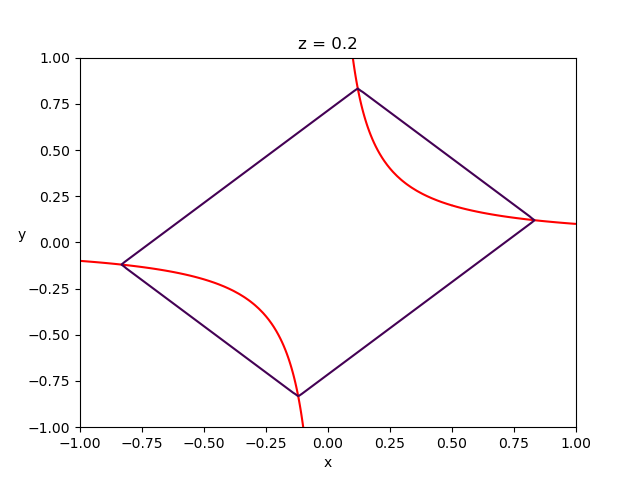
\includegraphics[scale=.3]{hw7 level curves z = 0.2}
		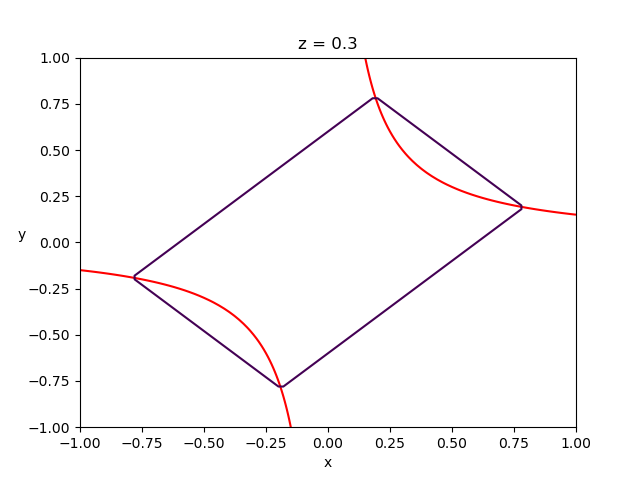
\includegraphics[scale=.3]{hw7 level curves z = 0.3}
		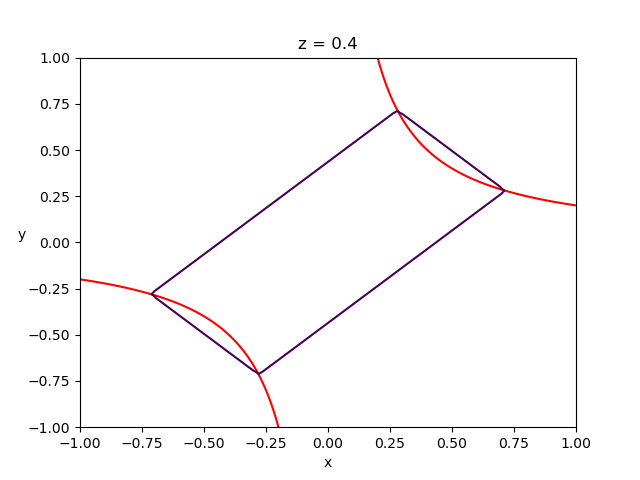
\includegraphics[scale=.3]{hw7 level curves z = 0.4}
	\end{center}
	
	
	
	\pagebreak
	
	
	
	\item
	
	
	
\end{enumerate}
	
	
	
	
\end{document}